
\section{Contribuição}\label{sec:contribuicao}

Este capítulo apresenta o \emph{AIMD CUBIC}, controlador
adaptativo de taxa de bits proposto para o Sunshine. A
exposição segue cinco eixos: o recorte do problema e as
decisões de projeto que o delimitam; a visão geral da política
de controle; o detalhamento do algoritmo de detecção e atuação;
a justificativa para a cadência de decisão e o uso de
histerese; e, por fim, a descrição da integração do controlador
na arquitetura do Sunshine.

\subsection{Recorte do Problema}

A política de controle proposta foi delimitada por três decisões de projeto que precedem qualquer escolha algorítmica. A primeira estabelece que toda a lógica opera no servidor, utilizando apenas sinais já disponíveis no Sunshine, sem modificações no protocolo Moonlight nem cooperação adicional do cliente. Essa restrição é motivada por questões práticas: o Sunshine compartilha o protocolo com clientes Moonlight de terceiros, cuja evolução está fora do controle do projeto, tornando inviável qualquer requisito de extensão. A segunda decisão é a adoção do RTT como sinal único, em contraposição a métricas que exigiriam sincronização de relógio ou \emph{feedback} adicional por quadro. O RTT é mantido continuamente pela biblioteca ENet no canal de controle e já é exposto pelo Sunshine, o que o torna o sinal de menor custo operacional disponível.

A terceira decisão consiste em priorizar métricas de cauda da distribuição de latência, como picos, p99 e eventos de \emph{stall}, em detrimento de medidas centrais como a mediana (p50). Essa escolha decorre da assimetria de QoE discutida no Capítulo~\ref{sec:referencial}: ganhos acima do patamar de saturação do MOS são marginais, enquanto degradações abaixo dele comprometem significativamente a jogabilidade.

Esse recorte diferencia diretamente o presente trabalho do
estado da arte mais próximo. O C\textsuperscript{3}G de Alós et
al.~\cite{alos2019} também opera no servidor, mas depende do
envio de confirmação por quadro de vídeo, exigindo extensão do
protocolo. O ABRAGame de Armendariz e
Joskowicz~\cite{abragame} opera majoritariamente no cliente e
pressupõe sincronização de relógio para o cálculo de atraso
unidirecional. O GCC de Carlucci et al.~\cite{gcc} opera por
pacote sobre \emph{feedback} RTCP contínuo, granularidade
incompatível com o canal de controle do Moonlight. Cada uma
dessas abordagens é viável em seu ambiente original; nenhuma é
diretamente transplantável ao Sunshine sem custos arquiteturais
substanciais.

\subsection{Visão Geral do Controlador}

O \emph{AIMD CUBIC} é uma política de controle baseada em \emph{Additive Increase, Multiplicative Decrease} (AIMD), complementada por dois mecanismos do algoritmo CUBIC~\cite{cubic}: a curva cúbica de recuperação após reduções de taxa e o mecanismo de \emph{fast convergence} para atualização do teto de referência. O controlador é organizado como uma máquina de estados composta por cinco estados (estável, congestionado, decrescendo, recuperando e sondando), sendo avaliado periodicamente a partir de amostras de RTT obtidas durante a transmissão.

As amostras de RTT são coletadas continuamente ao longo da transmissão e utilizadas para atualizar os contadores de duração contínua acima e abaixo dos limiares configurados. As decisões de controle, entretanto, são tomadas em uma cadência fixa de 1~Hz, desacoplada da taxa de quadros do codificador. Em cada ciclo de decisão, o controlador determina se a taxa de bits-alvo deve ser mantida, reduzida ou aumentada. Reduções são disparadas quando o RTT permanece acima do limiar por um intervalo correspondente à histerese configurada, enquanto aumentos ocorrem após períodos sustentados abaixo do limiar e seguem a curva cúbica do CUBIC para definir a magnitude do incremento.


\begin{figure}[!t]
  \centering
  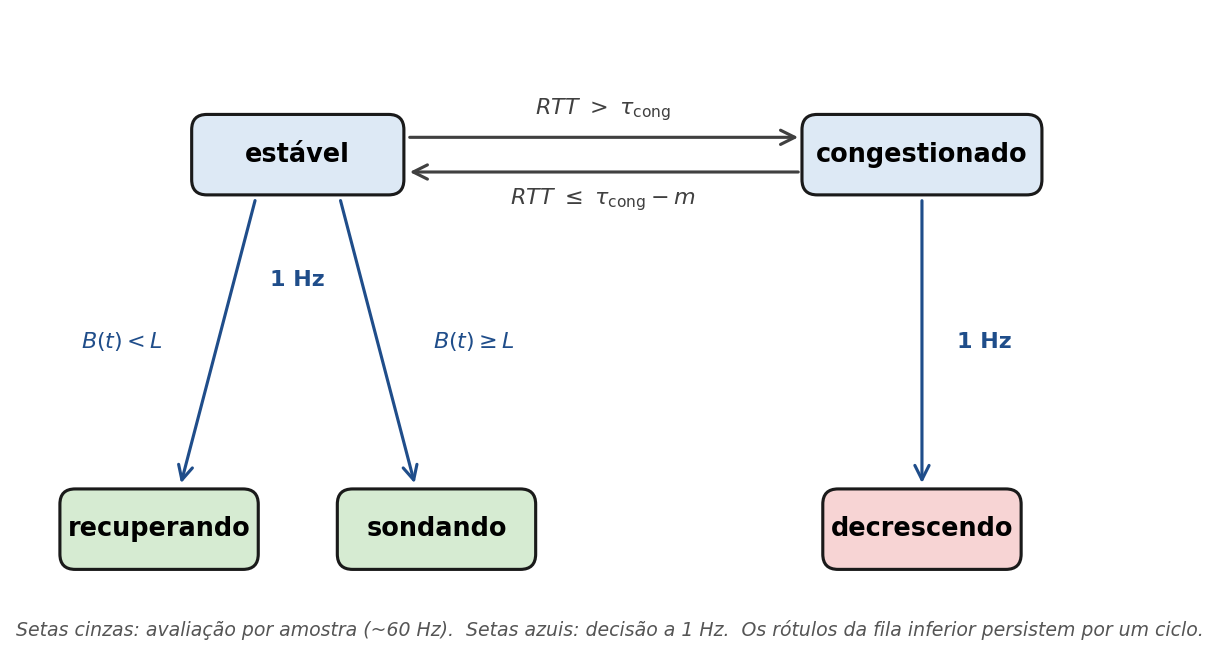
\includegraphics[width=\columnwidth]{images/state_machine.png}
  \caption{Máquina de estados do controlador AIMD CUBIC. A
  cada amostra de RTT (setas cinzas), o controlador transita
  entre os estados \emph{estável} e \emph{congestionado}
  conforme o RTT ultrapassa o limiar $\tau_{\rm cong}$ ou
  retorna abaixo de $\tau_{\rm cong} - m$, onde $m$ é a margem
  de histerese. A cada ciclo de decisão a 1~Hz (setas azuis),
  e desde que o \emph{streak} de duração mínima associado
  ($h_{\rm down}$ para decrementos, $h_{\rm up}$ para
  incrementos) tenha sido acumulado, o controlador atua sobre
  a taxa de bits-alvo do codificador: \emph{decrescendo} a
  partir de \emph{congestionado}; \emph{recuperando} ou
  \emph{sondando} a partir de \emph{estável}, conforme a
  amostra $B(t)$ da curva cúbica de recuperação esteja abaixo
  ou acima do teto $L$. Os rótulos da fila inferior persistem
  até o próximo ciclo de decisão.}
  \label{fig:state-machine}
\end{figure}

\subsection{Algoritmo}

\subsubsection{Sinal e Detecção}

O controlador recebe, a cada quadro codificado, uma amostra de
RTT proveniente da biblioteca ENet. A partir dessa amostra, dois
contadores de duração são mantidos. O primeiro, denominado
\emph{streak} de congestão, registra o início da janela contínua
mais recente em que o RTT permanece acima do limiar de
referência $\tau_{\text{cong}}$; é reiniciado sempre que uma
amostra retorna a valores aceitáveis. O segundo, denominado
\emph{streak} de via livre, registra simetricamente o início da
janela contínua em que o RTT permanece abaixo de
$\tau_{\text{cong}} - m$, onde $m$ é uma margem de histerese
introduzida pela razão discutida adiante. Os dois contadores são
atualizados continuamente, mas não disparam decisões por si só.

\subsubsection{Decremento Multiplicativo com \emph{Fast Convergence}}

Quando o \emph{streak} de congestão atinge uma duração mínima
$h_{\text{down}}$, o controlador aplica uma redução
multiplicativa à taxa atual:
\begin{equation}
  \text{kbps}_{\text{novo}} \gets \max\!\left( \beta \cdot \text{kbps}, \text{kbps}_{\min} \right)
  \label{eq:decrease}
\end{equation}
onde $\beta \in (0,1)$ é o fator de retenção e
$\text{kbps}_{\min}$ é o piso de operação. Empregamos $\beta = 0{,}7$,
valor utilizado no controlador AIMD de referência e mantido
nesta versão para isolar o efeito das demais alterações.

Antes da redução propriamente dita, o teto de recuperação
$L$ (último valor conhecido considerado seguro) é atualizado.
Em condições normais, em que a taxa atual ainda corresponde ao
último patamar estável, $L$ recebe o valor da taxa atual. Em
condições de congestionamento persistente, em que uma nova
redução é disparada antes que o controlador tenha recuperado o
patamar anterior, situação caracterizada por
$\text{kbps} < L$ no instante do disparo, $L$ é atualizado
segundo o mecanismo de fast convergence do
CUBIC:
\begin{equation}
  L \gets \text{kbps} \cdot \frac{1 + \beta}{2}
  \label{eq:fastconv}
\end{equation}
Esse ajuste retira do controlador a expectativa de retornar a
um teto que se mostrou inalcançável, fazendo-o convergir para
uma estimativa progressivamente mais próxima da capacidade
efetiva do canal. Em cenários de constrição prolongada, o
mecanismo evita que a curva de recuperação descrita a seguir
fique perpetuamente apontando para um valor obsoleto.

\subsubsection{Curva de Recuperação Cúbica}

Quando o \emph{streak} de via livre atinge uma duração mínima
$h_{\text{up}}$, o controlador aplica um incremento à taxa
atual. A magnitude do incremento é determinada por uma
amostragem da curva cúbica de recuperação do
CUBIC~\cite{cubic}:
\begin{equation}
  B(t) = C \cdot (t - K)^3 + L
  \label{eq:cubic-controller}
\end{equation}
onde $t$ é o tempo decorrido em segundos desde a última
redução, $L$ é o teto de recuperação definido por
(\ref{eq:fastconv}), $K$ é o tempo nominal de recuperação até
$L$, e $C = (1 - \beta) \cdot L / K^3$. A nova taxa-alvo é
$B(t)$, restrita ao intervalo $[\text{kbps},
\text{kbps}_{\max}]$, de modo que a curva nunca conduz a uma
redução, apenas a manutenção ou crescimento.

A forma de $B(t)$ é a mesma do CUBIC original, descrita no
Capítulo~\ref{sec:referencial}: côncava para $t < K$,
recuperando rapidamente em direção a $L$; aproximadamente
estável próximo de $t = K$; e convexa para $t > K$, sondando
de forma cautelosa, e depois acelerada, taxas acima do último
patamar conhecido. Para o presente trabalho, adotou-se
$K = 15$~s, valor calibrado empiricamente para que a fase de
sondagem inicie em uma escala compatível com a duração típica
de janelas de constrição nos cenários avaliados.

Variações na ancoragem temporal de $t$ e na regra de reinício do
\emph{streak} de via livre após crescimentos foram avaliadas
empiricamente, com resultados que motivam a forma adotada aqui;
essa análise é apresentada no
Capítulo~\ref{sec:resultados}, Seção~\ref{sec:sensibilidade}.

% [SUGESTÃO DE FIGURA] curva B(t) plotada para K=5s e K=15s
\begin{figure}[!t]
  \centering
  \includegraphics[width=\columnwidth]{figs/placeholder-cubic-curve}
  \caption{Curva de recuperação $B(t)$ amostrada pelo
  controlador AIMD CUBIC para dois valores do parâmetro $K$
  (\SI{5}{\second} e \SI{15}{\second}), com $\beta = 0{,}7$ e
  $L = 10\,000$~kbps. A região côncava ($t < K$) promove
  recuperação rápida em direção ao teto $L$; a região convexa
  ($t > K$) realiza sondagem cautelosa de capacidade adicional.}
  \label{fig:cubic-curve}
\end{figure}

\subsection{Cadência de Decisão e Histerese}

Duas decisões de projeto merecem justificativa explícita por
afetarem diretamente o comportamento dinâmico do controlador: a
cadência de avaliação a 1~Hz e o uso de histerese nos disparos
de decremento e incremento.

A cadência de 1~Hz é menor que a taxa de quadros do codificador
(tipicamente 60~Hz) por escolha deliberada. Reconfigurações
sucessivas e próximas no tempo da taxa do codificador
introduzem custos que vão da reinicialização de contextos
internos do \emph{encoder} ao envio de quadros IDR não
planejados, ambos potencialmente capazes de agravar a própria
condição de congestionamento que o controlador busca aliviar.
Espaçar as decisões em intervalos de um segundo permite que
cada atuação se propague pelo \emph{buffer} do gargalo e
manifeste seu efeito no RTT antes que a próxima decisão seja
tomada, evitando ciclos de realimentação curtos.

A histerese é um mecanismo clássico em sistemas de controle utilizado para evitar oscilações em torno de um limiar de decisão. No controlador proposto, ela é introduzida em dois níveis. Primeiro, exige-se que a condição de disparo (RTT sustentadamente acima ou abaixo do limiar) persista por uma duração mínima --- $h_{\text{down}}$ para decrementos e $h_{\text{up}}$ para incrementos --- antes que qualquer atuação ocorra. Esse requisito filtra picos transitórios de RTT, comuns em redes domésticas, que sob um critério instantâneo poderiam provocar uma sequência indesejada de cortes e recuperações.

Além disso, o controlador utiliza limiares distintos para identificar congestionamento e recuperação. Enquanto a entrada em congestionamento é caracterizada por RTT acima de $\tau_{\text{cong}}$, a condição de via livre exige que o RTT permaneça abaixo de $\tau_{\text{cong}}-m$, onde $m$ é uma margem de histerese. Dessa forma, pequenas oscilações do RTT em torno do limiar não fazem o controlador alternar continuamente entre os dois estados, permitindo que variações compatíveis com o ruído natural da rede sejam absorvidas sem disparar atuações desnecessárias.


Os valores adotados para todos os parâmetros do controlador são
sintetizados na Tabela~\ref{tab:params}. A escolha de cada
valor seguiu a calibração empírica conduzida ao longo do
desenvolvimento e descrita parcialmente no
Capítulo~\ref{sec:metodologia}.

\begin{table}[!t]
  \caption{Parâmetros do controlador AIMD CUBIC adotados na
  campanha experimental.}
  \label{tab:params}
  \centering
  \begin{tabular}{lll}
    \toprule
    \textbf{Parâmetro} & \textbf{Símbolo} & \textbf{Valor} \\
    \midrule
    Limiar de RTT (congestionamento) & $\tau_{\text{cong}}$ & \SI{100}{\milli\second} \\
    Margem de histerese & $m$ & \SI{20}{\milli\second} \\
    Histerese de decremento & $h_{\text{down}}$ & \SI{2000}{\milli\second} \\
    Histerese de incremento & $h_{\text{up}}$ & \SI{1000}{\milli\second} \\
    Fator de retenção & $\beta$ & 0{,}70 \\
    Tempo nominal de recuperação & $K$ & \SI{15}{\second} \\
    \emph{Fast convergence} & --- & ativo \\
    Intervalo de decisão & --- & \SI{1000}{\milli\second} \\
    Taxa mínima & $\text{kbps}_{\min}$ & \SI{1000}{\kilo\bit\per\second} \\
    Taxa máxima & $\text{kbps}_{\max}$ & inicial da sessão \\
    \bottomrule
  \end{tabular}
\end{table}

\subsection{Integração no Sunshine}

A política de controle foi implementada como uma classe
isolada em \texttt{src/bitrate\_controller.\{h,cpp\}}, contendo
exclusivamente lógica de decisão, sem qualquer acoplamento a
mecanismos de entrada ou saída do servidor. A classe expõe um
único método de atualização, \texttt{on\_sample}, que recebe
uma estrutura com a amostra de RTT corrente e retorna,
opcionalmente, uma nova taxa de bits-alvo quando uma decisão
de atuação é tomada. Essa separação preserva a testabilidade
do componente, viabilizando cobertura por testes unitários em
\emph{gtest} sob \texttt{tests/} sem necessidade de
infraestrutura de rede.

A integração com o restante do servidor ocorre em
\texttt{src/stream.cpp}, no laço principal de transmissão de
vídeo. A cada quadro codificado, a \emph{thread} de
\emph{broadcast} consulta o RTT corrente fornecido pela
biblioteca ENet e invoca \texttt{on\_sample}; quando o
controlador retorna uma nova taxa-alvo, a \emph{thread} aciona
o mecanismo de reconfiguração do codificador.

Os parâmetros do controlador foram expostos ao usuário em
\texttt{src/config.cpp}, junto aos demais parâmetros de
\emph{streaming}. A escolha de tornar os parâmetros
configuráveis, em vez de fixá-los no código, decorre da
expectativa de que diferentes perfis de uso, tipos de jogo e
condições típicas de rede do usuário possam exigir calibrações
próprias, e do reconhecimento de que a campanha
experimental conduzida neste trabalho cobre apenas um
subconjunto desses cenários. As mensagens visíveis ao usuário
adotam \texttt{boost::locale::translate} para internacionalização,
em conformidade com a convenção do projeto. O código segue as
diretrizes de formatação do \texttt{.clang-format} do
repositório e foi submetido como contribuição ao projeto
\emph{upstream}.
